\documentclass[12pt]{article}

\usepackage{sbc-template}
\usepackage{graphicx,url}
\usepackage[utf8]{inputenc}
\usepackage[english]{babel}
%\usepackage[latin1]{inputenc}  

\usepackage{booktabs} 
\usepackage{caption}

\newcommand{\starflet}{\textbf{Star-Fletcher}}
\newcommand{\waveprop}{\texttt{wave\_propagation}}
\newcommand{\waveinsert}{\texttt{wave\_insertion}}
\newcommand{\blockwrite}{\texttt{write\_block}}

\sloppy

\title{How STF allows trivial overlap of \\ I/O and computations on Forward RTM}

\author{Pedro Henrique Boniatti Colle, Lucas Mello Schnorr}

\address{Instituto de Informática -- Universidade Federal do Rio Grande do Sul
  (UFRGS)\\
  Caixa Postal 15.064 -- 91.501-970 -- Porto Alegre -- RS -- Brazil
  \email{\{phbcolle,schnorr\}@inf.ufrgs.br}
}

\begin{document} 

\maketitle

\begin{abstract}
	With the evermore complex ecosystem of High Performance Computing (HPC), the Sequential Task Flow (STF) model arrives to provide a convenient interface to compute in heterogeneous architectures. This paper presents \starflet, a Reverse Time Migration (RTM) program implemented using STF alongside time tiling which resulted in the side effect of complete I/O to disk masking.
\end{abstract}

\section{Introduction}
\label{sec:introduction}
	It's the end days of homogeneous architectures. With the ever-increasing computing demands of High Performance Computing (HPC) applications, nodes in data centers are required to incorporate increasingly different hardware accelerators, even more after the AI boom. This increases the complexity of writing programs that uses all the resource in a node.

	One of the answers for this problem are Sequential Task Flow (STF) runtime systems. In those, work is segmented in tasks with explicit dependencies. Those tasks are submitted sequentially and execute asynchronously with respect to their dependencies. With this model it is easy to distribute task between different architectures. One could implement a task to run in the CPU and also provide an implementation to run in the GPU. The runtime handles the load balancing and data transfers. Some popular runtimes are PaRSEC \cite{bosilca_parsec_2013} and StarPU \cite{starpu-paper}, the latter was used in this paper. 
	Both of these systems have a data management side, which allows for easier tracking of dependencies and task submission. StarPU's automatic memory management was essential in enabling many mechanisms for this paper's program optimizations. Many applications adopted this paradigm for a plethora of contexts, like dense linear algebra \cite{abdulah_accelerating_2022}, Computational Fluid Dynamics (CFD) \cite{couteyen_carpaye_design_2018,leandro_nesi_task-based_2020} and Reverse Time Migration (RTM) applications \cite{boillot_task-based_2014, alonazi_asynchronous_2019}.

	RTM is a tool of seismic analysis for detecting subsurface deposits of materials. It propagates a wavefield forwards in time, records it and then integrates the recording back in time to generate a partial image. This process is repeated many times, each called a \textit{shot}, to generate the final visualization. There are no dependencies between \textit{shots}, making RTM applications embarrassingly parallel. The Fletcher algorithm \cite{fletcher_reverse_2009} can deal with Tilted Transverse Isotropic (TTI) medium and is the chosen implementation of this paper's program.

	One important characteristic of RTM is that it's recorded data between the forwards and backwards propagation can be massive. A normal volume of $1000 \times 1000 \times 500$ saved in FP64 results in $~4\;GB$ of data, which is saved many times during execution. That makes this kind of application I/O bound. Modern research focuses in overlapping computation with I/O operations \cite{alonazi_asynchronous_2019, kunas_enhancing_2025}. AlOnazi's work calls back to the STF paradigm, in which the StarPU runtime system was used to manage the I/O and data transfer operations while the computation was done in GPUs. This utilization was limited to homogenous computation on GPUs and two-level parallelism, where the whole medium was placed in the GPUs shared memory. This resulted in a two-tier parallel system, where computations used traditional parallel methods while the I/O used the STF model.

	In order to fill this design space, we propose \starflet, a first-order task parallelism with space-segmentation implementation of Fletcher using the StarPU library. It represents only the forwards wave propagation, with the snapshots being saved to disk in order to always simulate a medium too large to fit in main memory. The decision of space segmentation allows for first-order task parallelism while enabling spaces too large to fit in memory to be processed efficiently. We utilize the works of \cite{leandro_nesi_task-based_2020,qu_exploiting_2023} to implement time tiling in order to incur speed-ups with respect to cache reuse. By reformulating \starflet \, to fit this paradigm, all I/O operations became masked behind computation. This side effect was possible because STF, and  especially StarPU, are extremely well-equipped to implement the time tiling paradigm.

	In the section \ref{sec:methodsandmaterials} it is discussed the implementation detail of \starflet, in section \ref{sec:parcialresults} it is present partial results of overlap of I/O and computation and in section \ref{sec:conclusion} it is elaborated future directions for the project and which experimental results are being aimed for.

\section{Methods and Materials}
\label{sec:methodsandmaterials}
	In Fletcher's basic implementation, two buffers are used, the current and the previous. The current is used to compute the values that will be added to the previous, akin to $prev +\!\!= F(curr)$. Then the buffers are swapped, and the process repeats until all iterations are executed. This format stops time tiling because it requires that an iteration completely finishes before starting the next one. To enable time tiling, the swap was removed, resulting in the computation $A_{t} := F(A_{t-1}) + A_{t-2}$. This relies on StarPU's automatic memory management\footnote{Chapter 27.2 of StarPU's manual \url{https://files.inria.fr/starpu/doc/html/AdvancedDataManagement.html}}. With $A_{t}$ as an exclusively write dependency, StarPU can allocate it when necessary and free it when no other task requires it. This mechanism allows for time tiling to comprise as many iterations as the system's memory allows. Another consequence is that writing $prev$ to disk, or in this case $A_t$, does not block the computation of the next iteration anymore, allowing for asynchronous I/O.

	We have implemented three tasks in StarPU to implement time tiling : \waveprop, \waveinsert\,and \blockwrite. The space segmentation required disjointed memory, which required additional bounds checks when accessing neighboring blocks in the \waveprop\, task. Using meta programming, the number of checks were reduced to three in the cross product and two in the second derivative. The disjointed space also affected \blockwrite\, task. For it, each thread used its own file and wrote the received blocks in them with some metadata that enables later reconstruction of the full volume. Currently, on program termination, a script congeals all these files into one, which will be integrated in the final application. 

\section{Preliminary Results}
\label{sec:parcialresults}
	%experimentos rodados na CEI1.
	The program was tested in one of the nodes of the 'cei' partition of INF/UFRGS's PCAD platform (2x Intel(R) Xeon(R) Silver 4116 CPUs 2.1 GHz, 48 threads, 24 cores). A volume of $600 \times 600 \times 600$ was iterated 10 times, snapshooting at various interval configurations. To illustrate the I/O masking, Figure \ref{img:graph} represents the execution where the space was divided in 64 blocks and, at each step, the full volume was saved to disk. The $y$ axis represent interations and $x$ axis time. The blocks are represented as vertical lines in each iteration, but they are represented so close together that it appears as a bar.

\begin{figure}[ht]
    \centering
	% trim order: Left, Bottom, Right, Top
    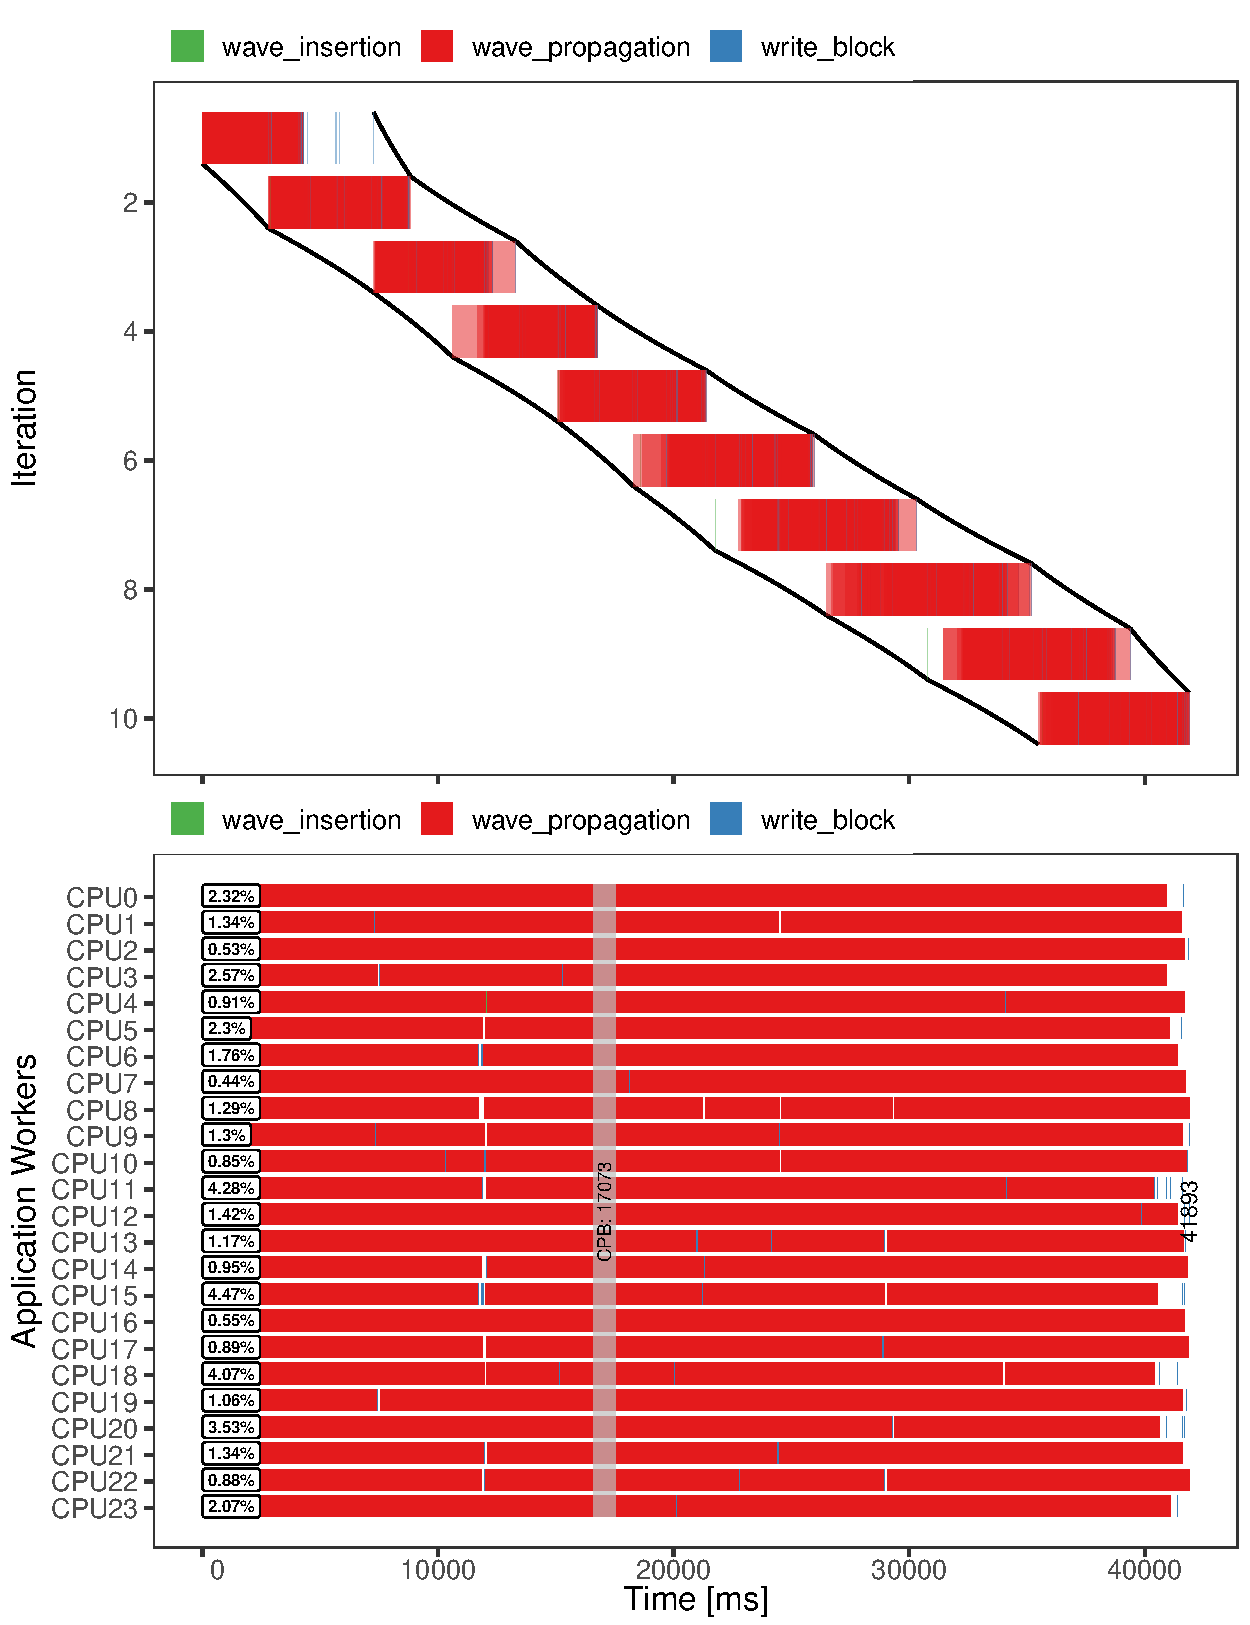
\includegraphics[page=1, trim=0cm 14.38cm 0cm 0cm, clip, width=\textwidth, height=0.25\textheight]{imgs/trace_560_1_4_0_starvz.pdf}
    \caption{Trace showing the parallelization of tasks per iteration.}
	\label{img:graph}
\end{figure}

Barely any \blockwrite\, is visible in Figure \ref{img:graph}. This shows that it is being interleaved with the computation and is not part of the execution's critical path at any point. We can analyze the data in Table \ref{tab:iobench} to see that each I/O task does not comprise a big individual expense. Scattering them throughout computation results in an effective performance gain. 
	
\begin{table}[ht]
    \centering
    \caption{Amount of Tasks executed with their Mean, Min and Max execution time in milliseconds.}
    \label{tab:iobench}
    \begin{tabular}{lrrrr}
        \toprule
        Task & Amount & Mean & Min & Max \\
        \waveinsert & 50 & 2.9 & 1.83 & 6.33 \\
        \waveprop & 3200 & 99100 & 55100 & 451000 \\
        \blockwrite & 704 & 39.5 & 13.9 & 628 \\
        \bottomrule
    \end{tabular}
\end{table}

\section{Conclusion and Future Work}
\label{sec:conclusion}

	The ease of implementing time tiling in \starflet\, was only possible due to the STF model. StarPU's features allow for an easy implementation and as a bonus it breaks dependencies that stop I/O masking. Nonetheless, this program is a work in progress and more comparisons with conventional parallel versions of fletcher are necessary to validate \starflet\,performance. It's still necessary to explore if the time tiling design really results in performance gains and in cache reuse.

\bibliographystyle{sbc}
\bibliography{references.bib}

\end{document}
